\documentclass[a4paper]{article}% Formato de plantill

\usepackage[utf8]{inputenc}
\usepackage[spanish]{babel}
\usepackage[margin=2cm, top=2cm, includefoot]{geometry}
\usepackage{graphicx} %Para agregar imagenes
\usepackage[table,xcdraw]{xcolor} %Para los colores
\usepackage[most]{tcolorbox} %Para la inserción de cuadros en la portada
\usepackage{fancyhdr} %Define el estilo de la pagina
\usepackage[hidelinks]{hyperref} %Gestión de hipervinculos
\usepackage{parskip} %Tabulación del documento
\usepackage[figurename=Figura]{caption} %Cambiar el nombre de las imagenes
\usepackage{smartdiagram} %Para agregar diagramas
\usepackage{listings} %Agregar codigo en el documento
\usepackage{zed-csp} %Agregar tablas
\usepackage{tabularx}	% Para la tabla inicial

%Declaración de colores
\definecolor{greenPortada}{HTML}{69A84F}

%Declaración de variables
\newcommand{\LogoPortada}{Imagenes/portada.png} %Imagen de portada
\newcommand{\NombreMaquina}{(Nombre)} %Nombre de la maquina
\newcommand{\LogoMaquina}{Imagenes/Previse.png} %Icono de la maquina

%Adicionales
\addto\captionsspanish{\renewcommand{\contentsname}{Contenido}} %Cambio del formato del indice
\setlength{\headheight}{40.2pt} %Manejar el indice de la pagina (Imagenes izquiera y derecha)
\pagestyle{fancy}
\fancyhf{}
\lhead{
\includegraphics[width=5cm]{Imagenes/portada.png}} %Imagen Izquierda
\rhead{
\includegraphics[height=1.5cm]{Imagenes/Previse.png}} %Imagen Derecha
\renewcommand{\headrulewidth}{3pt} %Barra abajo de las imagenes
\renewcommand{\headrule}{\hbox to\headwidth{\color{greenPortada}\leaders\hrule height \headrulewidth\hfill}}
\renewcommand{\lstlistingname}{Codigo} %Para cambiar el nombre de los codigos
%Agregar color al codigo
\definecolor{codegreen}{rgb}{0,0.6,0}
\definecolor{codegray}{rgb}{0.5,0.5,0.5}
\definecolor{codepurple}{rgb}{0.58,0,0.82}
\definecolor{backcolour}{rgb}{0.95,0.95,0.92}

\lstdefinestyle{mystyle}{
    backgroundcolor=\color{backcolour},   
    commentstyle=\color{codegreen},
    keywordstyle=\color{magenta},
    numberstyle=\tiny\color{codegray},
    stringstyle=\color{codepurple},
    basicstyle=\ttfamily\footnotesize,
    breakatwhitespace=false,         
    breaklines=true,                 
    captionpos=b,                    
    keepspaces=true,                 
    numbers=left,                    
    numbersep=5pt,                  
    showspaces=false,                
    showstringspaces=false,
    showtabs=false,                  
    tabsize=2
}
\lstset{style=mystyle} 
%-------------------------------

%Config para la tabla de la portada
\newcolumntype{Y}{>{\centering\arraybackslash}X}
\tcbset{tab1/.style={fonttitle=\bfseries\large,fontupper=\normalsize\sffamily,
		colback=white!10!white,
		colframe=greenPortada!75!black,
		colbacktitle=greenPortada!40!white,
		coltitle=black,
		center title,
		freelance,
		frame code={
			\foreach \n in {north east,north west,south east,south west}
			{\path [fill=greenPortada!75!black] (interior.\n) circle (2mm); };},}}
%--------------------------------------

%Comienzo del documento
\begin{document}
  \cfoot{\thepage}
   %Creación de portada
  \begin{titlepage}
  \centering
  \includegraphics[width=0.8\textwidth]{\LogoPortada}\par\vspace{0,8cm} %Incluir imagenes
   {\scshape\LARGE\textbf{Informe Técino}\par\vspace{0,2cm}}
   {\Huge\bfseries\textcolor{greenPortada}{Máquina \NombreMaquina}\par}
   \vfill\vfill
   %Logo de la Maquina
   \includegraphics[width=\textwidth,height=10cm, keepaspectratio]{\LogoMaquina}\par\vspace{1cm}
   \vfill
   %Cuadro de colores
    \begin{tcolorbox}[tab1,tabularx={Y||Y}]	
			{\Huge\bfseries{Dificultad}} & {\Huge\bfseries{IP}} \\ \\
			{\Large{Nivel}}  & {\Large{127.0.0.1}} \\
			\\
		\end{tcolorbox}
    \centering
   \vfill
   
   %Final de la portada -----------------------------------------------
   %Comienzo del Indice
   \clearpage
   \tableofcontents
   \clearpage
   %-------------------------------------------------------------------

   %Agregar una nueva sección al Contenido
   \raggedright %Poner un texto a lado derecho
   \section{Obtención de Información} 
   Esto es una plantilla para crear WriteUps sobre máquinas en Hack The Box {\textbf{\NombreMaquina}} de la plataforma \href{https://hackthebox.eu}{\textbf{\color{blue}HackTheBox}}
   \vspace{0.2cm}
    \begin{figure}[h] %Agregar imagen
        \centering
        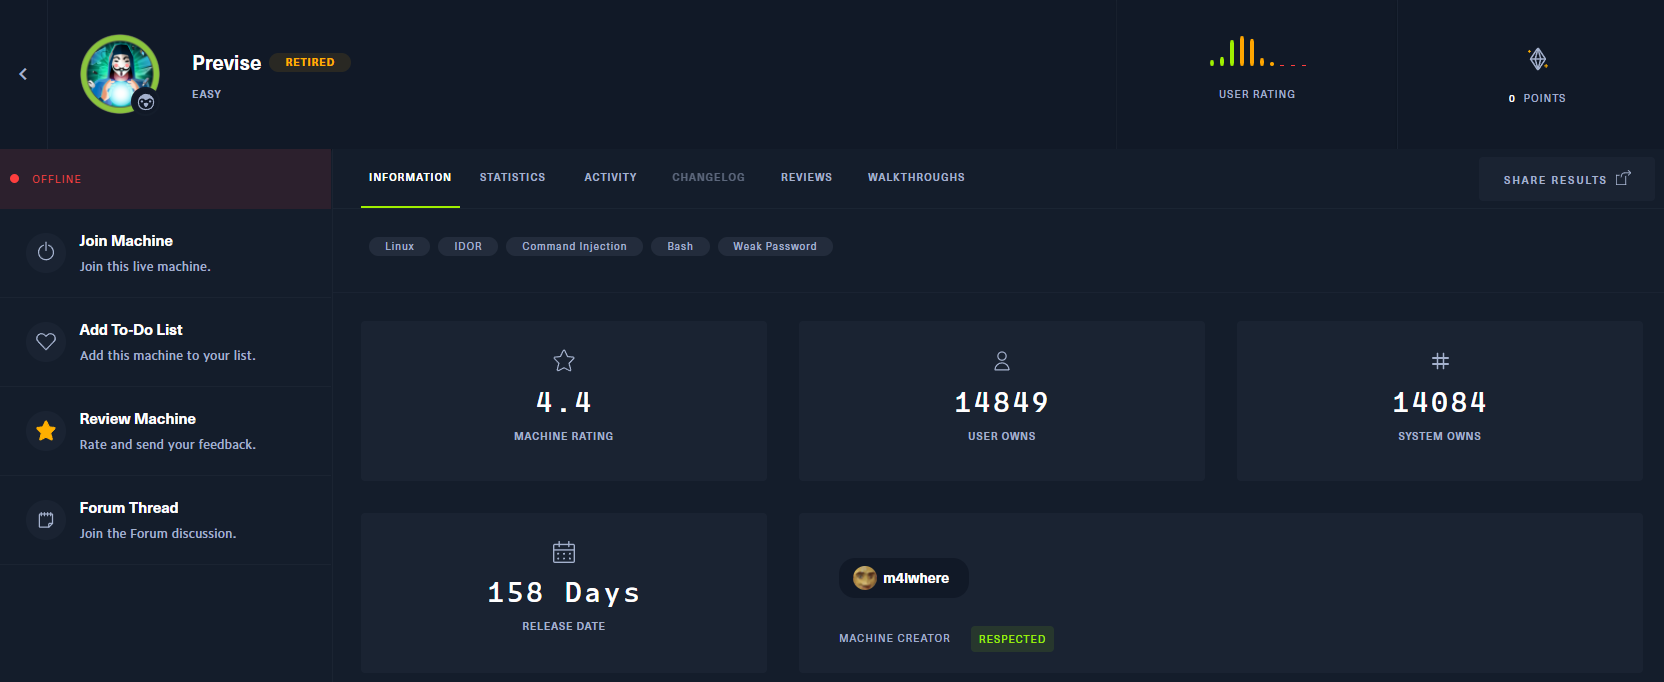
\includegraphics[width=\textwidth]{Imagenes/Detalles.png}
        \caption{Detalles de la Máquina}
        \label{fig:detalles}
    \end{figure} 
  %---------------------------------------------------------------------

  \section{Análisis} %Agregar otra sección al Contenido
   Un análisis sobre los información encontrada.
   \subsection{Info} %Crear una subcategoria
   Esto es una plantilla la cual puede ser modificada para crear writeup propios.
   
   \begin{figure}[h] %Crear un diagrama
      \begin{center}
      \smartdiagram[priority descriptive diagram]{
      a,
      b,
      c,
      d
      }
      \caption{Flujo de trabajo}
      \label{fig:diagrama}
      \end{center}
   \end{figure}
   %--------------------------------------------------------------------
   
   \section{Explotación} %Agregar otra sección al Contenido
    \subsection{Info}
    \vspace{0.1cm}
     Sección en la cual puede pegar codigo con su respectivo interprete \textbf{Python}
    \vspace{0.1cm}
    
    %Agregar codigo con colores
    \begin{lstlisting}[language=Python, caption=Script personalizado para los puertos abiertos] 
    num = int(input('Introduzca un numero: '))
    ifnum % 2 == 0:
    print('Par')
    else:
    print('Impar')
    \end{lstlisting}

    \vspace{0.2cm}
    Tablas para agregar mas información

    %Agregar una tabla
    \begin{schema}{TCP} 
       Info
       \where
       Info, aquí
    \end{schema}
    
 \vspace{0.1cm}
   
   %Redirigir a otra tabla o imagen
   Aquí se puede redirigir a la figura \ref{fig:detalles} de la página \pageref{fig:detalles}.
   
   
%Fin del Documento
  \end{titlepage}
\end{document}